\documentclass[journal,12pt,twocolumn]{IEEEtran}
%
\usepackage{setspace}
\usepackage{gensymb}
%\doublespacing
\singlespacing

%\usepackage{graphicx}
%\usepackage{amssymb}
%\usepackage{relsize}
\usepackage[cmex10]{amsmath}
%\usepackage{amsthm}
%\interdisplaylinepenalty=2500
%\savesymbol{iint}
%\usepackage{txfonts}
%\restoresymbol{TXF}{iint}
%\usepackage{wasysym}
\usepackage{amsthm}
\usepackage{iithtlc}
\usepackage{mathrsfs}
\usepackage{txfonts}
\usepackage{stfloats}
\usepackage{bm}
\usepackage{cite}
\usepackage{cases}
\usepackage{subfig}
%\usepackage{xtab}
\usepackage{longtable}
\usepackage{multirow}
%\usepackage{algorithm}
%\usepackage{algpseudocode}
\usepackage{enumitem}
\usepackage{mathtools}
\usepackage{tikz}
\usepackage{circuitikz}
\usepackage{verbatim}
\usepackage{tfrupee}
\usepackage[breaklinks=true]{hyperref}
%\usepackage{stmaryrd}
\usepackage{tkz-euclide} % loads  TikZ and tkz-base
%\usetkzobj{all}
\usepackage{listings}
    \usepackage{color}                                            %%
    \usepackage{array}                                            %%
    \usepackage{longtable}                                        %%
    \usepackage{calc}                                             %%
    \usepackage{multirow}                                         %%
    \usepackage{hhline}                                           %%
    \usepackage{ifthen}                                           %%
  %optionally (for landscape tables embedded in another document): %%
    \usepackage{lscape}     
\usepackage{multicol}
\usepackage{chngcntr}
%\usepackage{enumerate}

%\usepackage{wasysym}
%\newcounter{MYtempeqncnt}
\DeclareMathOperator*{\Res}{Res}
%\renewcommand{\baselinestretch}{2}
\renewcommand\thesection{\arabic{section}}
\renewcommand\thesubsection{\thesection.\arabic{subsection}}
\renewcommand\thesubsubsection{\thesubsection.\arabic{subsubsection}}

\renewcommand\thesectiondis{\arabic{section}}
\renewcommand\thesubsectiondis{\thesectiondis.\arabic{subsection}}
\renewcommand\thesubsubsectiondis{\thesubsectiondis.\arabic{subsubsection}}

% correct bad hyphenation here
\hyphenation{op-tical net-works semi-conduc-tor}
\def\inputGnumericTable{}                                 %%

\lstset{
%language=C,
frame=single, 
breaklines=true,
columns=fullflexible
}
%\lstset{
%language=tex,
%frame=single, 
%breaklines=true
%}

\begin{document}
%


\newtheorem{theorem}{Theorem}[section]
\newtheorem{problem}{Problem}
\newtheorem{proposition}{Proposition}[section]
\newtheorem{lemma}{Lemma}[section]
\newtheorem{corollary}[theorem]{Corollary}
\newtheorem{example}{Example}[section]
\newtheorem{definition}[problem]{Definition}
%\newtheorem{thm}{Theorem}[section] 
%\newtheorem{defn}[thm]{Definition}
%\newtheorem{algorithm}{Algorithm}[section]
%\newtheorem{cor}{Corollary}
\newcommand{\BEQA}{\begin{eqnarray}}
\newcommand{\EEQA}{\end{eqnarray}}
\newcommand{\define}{\stackrel{\triangle}{=}}

\bibliographystyle{IEEEtran}
%\bibliographystyle{ieeetr}


\providecommand{\mbf}{\mathbf}
\providecommand{\pr}[1]{\ensuremath{\Pr\left(#1\right)}}
\providecommand{\qfunc}[1]{\ensuremath{Q\left(#1\right)}}
\providecommand{\sbrak}[1]{\ensuremath{{}\left[#1\right]}}
\providecommand{\lsbrak}[1]{\ensuremath{{}\left[#1\right.}}
\providecommand{\rsbrak}[1]{\ensuremath{{}\left.#1\right]}}
\providecommand{\brak}[1]{\ensuremath{\left(#1\right)}}
\providecommand{\lbrak}[1]{\ensuremath{\left(#1\right.}}
\providecommand{\rbrak}[1]{\ensuremath{\left.#1\right)}}
\providecommand{\cbrak}[1]{\ensuremath{\left\{#1\right\}}}
\providecommand{\lcbrak}[1]{\ensuremath{\left\{#1\right.}}
\providecommand{\rcbrak}[1]{\ensuremath{\left.#1\right\}}}
\theoremstyle{remark}
\newtheorem{rem}{Remark}
\newcommand{\sgn}{\mathop{\mathrm{sgn}}}
\providecommand{\abs}[1]{\left\vert#1\right\vert}
\providecommand{\res}[1]{\Res\displaylimits_{#1}} 
\providecommand{\norm}[1]{\left\lVert#1\right\rVert}
%\providecommand{\norm}[1]{\lVert#1\rVert}
\providecommand{\mtx}[1]{\mathbf{#1}}
\providecommand{\mean}[1]{E\left[ #1 \right]}
\providecommand{\gauss}[2]{\mathcal{N}\ensuremath{\left(#1,#2\right)}}
\providecommand{\fourier}{\overset{\mathcal{F}}{ \rightleftharpoons}}
%\providecommand{\hilbert}{\overset{\mathcal{H}}{ \rightleftharpoons}}
\providecommand{\system}{\overset{\mathcal{H}}{ \longleftrightarrow}}
	%\newcommand{\solution}[2]{\vec{Solution:}{#1}}
\newcommand{\solution}{\noindent \textbf{Solution: }}
\newcommand{\cosec}{\,\text{cosec}\,}
\providecommand{\dec}[2]{\ensuremath{\overset{#1}{\underset{#2}{\gtrless}}}}
\newcommand{\myvec}[1]{\ensuremath{\begin{pmatrix}#1\end{pmatrix}}}
\newcommand{\mydet}[1]{\ensuremath{\begin{vmatrix}#1\end{vmatrix}}}
%\numberwithin{equation}{section}
%\numberwithin{equation}{subsection}
%\numberwithin{problem}{section}
%\numberwithin{definition}{section}
\makeatletter
\@addtoreset{figure}{problem}
\makeatother

\let\StandardTheFigure\thefigure
\let\vec\mathbf
%\renewcommand{\thefigure}{\theproblem.\arabic{figure}}
\renewcommand{\thefigure}{\theproblem}
%\setlist[enumerate,1]{before=\renewcommand\theequation{\theenumi.\arabic{equation}}
%\counterwithin{equation}{enumi}


%\renewcommand{\theequation}{\arabic{subsection}.\arabic{equation}}

\def\putbox#1#2#3{\makebox[0in][l]{\makebox[#1][l]{}\raisebox{\baselineskip}[0in][0in]{\raisebox{#2}[0in][0in]{#3}}}}
     \def\rightbox#1{\makebox[0in][r]{#1}}
     \def\centbox#1{\makebox[0in]{#1}}
     \def\topbox#1{\raisebox{-\baselineskip}[0in][0in]{#1}}
     \def\midbox#1{\raisebox{-0.5\baselineskip}[0in][0in]{#1}}

\vspace{3cm}

\title{
	\logo{
Digital Modulation Techniques
	}
}
%\author{ C.~Shruti, P.~N.~V.~S.~S.~K.~ HAVISH, S.~S.~Ashish and G V V Sharma$^{*}$% <-this % stops a space
\author{ G V V Sharma$^{*}$% <-this % stops a space
	\thanks{*The author is with the Department
		of Electrical Engineering, Indian Institute of Technology, Hyderabad
		502285 India e-mail:  gadepall@iith.ac.in. All content in this manual is released under GNU GPL.  Free and open source.}
	
}	
%\title{
%	\logo{Matrix Analysis through Octave}{\begin{center}\includegraphics[scale=.24]{tlc}\end{center}}{}{HAMDSP}
%}


% paper title
% can use linebreaks \\ within to get better formatting as desired
%\title{Matrix Analysis through Octave}
%
%
% author names and IEEE memberships
% note positions of commas and nonbreaking spaces ( ~ ) LaTeX will not break
% a structure at a ~ so this keeps an author's name from being broken across
% two lines.
% use \thanks{} to gain access to the first footnote area
% a separate \thanks must be used for each paragraph as LaTeX2e's \thanks
% was not built to handle multiple paragraphs
%

%\author{<-this % stops a space
%\thanks{}}
%}
% note the % following the last \IEEEmembership and also \thanks - 
% these prevent an unwanted space from occurring between the last author name
% and the end of the author line. i.e., if you had this:
% 
% \author{....lastname \thanks{...} \thanks{...} }
%                     ^------------^------------^----Do not want these spaces!
%
% a space would be appended to the last name and could cause every name on that
% line to be shifted left slightly. This is one of those "LaTeX things". For
% instance, "\vec{A} \vec{B}" will typeset as "A B" not "AB". To get
% "AB" then you have to do: "\vec{A}\vec{B}"
% \thanks is no different in this regard, so shield the last } of each \thanks
% that ends a line with a % and do not let a space in before the next \thanks.
% Spaces after \IEEEmembership other than the last one are OK (and needed) as
% you are supposed to have spaces between the names. For what it is worth,
% this is a minor point as most people would not even notice if the said evil
% space somehow managed to creep in.



% The paper headers
%\markboth{Journal of \LaTeX\ Class Files,~Vol.~6, No.~1, January~2007}%
%{Shell \MakeLowercase{\textit{et al.}}: Bare Demo of IEEEtran.cls for Journals}
% The only time the second header will appear is for the odd numbered pages
% after the title page when using the twoside option.
% 
% *** Note that you probably will NOT want to include the author's ***
% *** name in the headers of peer review papers.                   ***
% You can use \ifCLASSOPTIONpeerreview for conditional compilation here if
% you desire.




% If you want to put a publisher's ID mark on the page you can do it like
% this:
%\IEEEpubid{0000--0000/00\$00.00~\copyright~2007 IEEE}
% Remember, if you use this you must call \IEEEpubidadjcol in the second
% column for its text to clear the IEEEpubid mark.



% make the title area
\maketitle

\newpage

\tableofcontents

\bigskip

\renewcommand{\thefigure}{\theenumi}
\renewcommand{\thetable}{\theenumi}
%\renewcommand{\theequation}{\theenumi}

%\begin{abstract}
%%\boldmath
%In this letter, an algorithm for evaluating the exact analytical bit error rate  (BER)  for the piecewise linear (PL) combiner for  multiple relays is presented. Previous results were available only for upto three relays. The algorithm is unique in the sense that  the actual mathematical expressions, that are prohibitively large, need not be explicitly obtained. The diversity gain due to multiple relays is shown through plots of the analytical BER, well supported by simulations. 
%
%\end{abstract}
% IEEEtran.cls defaults to using nonbold math in the Abstract.
% This preserves the distinction between vectors and scalars. However,
% if the journal you are submitting to favors bold math in the abstract,
% then you can use LaTeX's standard command \boldmath at the very start
% of the abstract to achieve this. Many IEEE journals frown on math
% in the abstract anyway.

% Note that keywords are not normally used for peerreview papers.
%\begin{IEEEkeywords}
%Cooperative diversity, decode and forward, piecewise linear
%\end{IEEEkeywords}



% For peer review papers, you can put extra information on the cover
% page as needed:
% \ifCLASSOPTIONpeerreview
% \begin{center} \bfseries EDICS Category: 3-BBND \end{center}
% \fi
%
% For peerreview papers, this IEEEtran command inserts a page break and
% creates the second title. It will be ignored for other modes.
%\IEEEpeerreviewmaketitle

\begin{abstract}
%\boldmath
The manual frames the problems of receiver design and performance analysis in digital communication as applications of probability theory.

\end{abstract}
% IEEEtran.cls defaults to using nonbold math in the Abstract.
% This preserves the distinction between vectors and scalars. However,
% if the journal you are submitting to favors bold math in the abstract,
% then you can use LaTeX's standard command \boldmath at the very start
% of the abstract to achieve this. Many IEEE journals frown on math
% in the abstract anyway.

% Note that keywords are not normally used for peerreview papers.
%\begin{IEEEkeywords}
%Cooperative diversity, decode and forward, piecewise linear
%\end{IEEEkeywords}



% For peer review papers, you can put extra information on the cover
% page as needed:
% \ifCLASSOPTIONpeerreview
% \begin{center} \bfseries EDICS Category: 3-BBND \end{center}
% \fi
%
% For peerreview papers, this IEEEtran command inserts a page break and
% creates the second title. It will be ignored for other modes.
\IEEEpeerreviewmaketitle

Download all codes in this manual from 
\begin{lstlisting}
svn co https://github.com/gadepall/comm/trunk/modulation/manual/codes
\end{lstlisting}

\renewcommand{\theequation}{\theenumi}
\section{BPSK}
\begin{enumerate}[label=\thesection.\arabic*.,ref=\thesection.\theenumi]
\numberwithin{equation}{enumi}

\item The {\em signal constellation diagram} for BPSK is given by Fig. \ref{fig:ee18btech11042_bpsk_const}.  The symbols $s_0$ and $s_1$ are equiprobable.  $\sqrt{E_b}$ is the energy transmitted per bit. Assuming a zero mean additive white gaussian noise (AWGN) with variance $\frac{N_0}{2}$,
obtain the symbols that are received.
%
\begin{figure}[!ht]
\centering
\resizebox{\columnwidth}{!}{\begin{circuitikz}[american]


    \ctikzset{tripoles/mos style/arrows}
    \draw[<->] (-5,0)--(5,0)node[right]{$x$};
    
    \filldraw[black](-2.5,0) circle(2pt) node[below] {$s_1$};
    \filldraw[black](2.5,0) circle(2pt) node[below] {$s_0$};
    \filldraw[black](0,0) circle(2pt) node[below] {$o$};
    
    
    
    
    
    
    
    
    
    
    
    
    
    
    \end{circuitikz}}
%\includegraphics[width=\columnwidth]{./ee18btech11042/figs/constellation.eps}
\caption{}
\label{fig:ee18btech11042_bpsk_const}
\end{figure}
%\begin{figure}[!ht]
%		\resizebox{\columnwidth}{!}{\begin{circuitikz}[american]


    \ctikzset{tripoles/mos style/arrows}
    \draw[<->] (-5,0)--(5,0)node[right]{$x$};
    
    \filldraw[black](-2.5,0) circle(2pt) node[below] {$s_1$};
    \filldraw[black](2.5,0) circle(2pt) node[below] {$s_0$};
    \filldraw[black](0,0) circle(2pt) node[below] {$o$};
    
    
    
    
    
    
    
    
    
    
    
    
    
    
    \end{circuitikz}}
%\caption{Constellation diagram}
%\label{fig:ee18btech11042_ee18btech11042_1}
%\end{figure}
\\
\solution The possible received symbols are
\begin{align}
y|s_0 &= \sqrt{E_b} + n
\\
y|s_1 &= -\sqrt{E_b} + n
\end{align}
%
where the AWGN $n \sim \gauss{0}{\frac{N_0}{2}}$.
%
\item

\label{prob:bpsk_decision}
From Fig. \ref{fig:ee18btech11042_bpsk_const} obtain a decision rule for BPSK
\solution The decision rule is
\begin{equation}
y \dec{s_0}{s_1} 0
\end{equation}

\item
Repeat the previous exercise using the MAP criterion.
\\
\solution
%Given symbols $s_0$ and $ s_1$ are equiprobable and assume symbol carries $\sqrt{E_b}$ per bit and consider a  additive white gaussian noise(AWGN) with mean 0 and variance $\frac{N_oN_0}{2}$ and take  symbols as equiprobable. The received symbols can be:
%\begin{align}
%    y|s_0 = \sqrt(E_b) + n
%    \label{eq:ee18btech11042_1}
%\end{align}
%\begin{align}
%    y|s_1 = -\sqrt(E_b) + n
%    \label{eq:ee18btech11042_2}
%\end{align}
According to MAP detection rule
%, we will decode the received signal  as symbol s for which  p\brak{s|y} is more.
\begin{align}
    \hat{s} &= \max_{s \in  \cbrak{s_0,s_1}} p\brak{s|y}
    \label{eq:ee18btech11042_3}
\\
    \implies p\brak{s_0|y} &\dec{s_0}{s_1} p\brak{s_1|y}
    \label{eq:ee18btech11042_4}
\end{align}
Using Bayes rule,
\begin{align}
    p\brak{s_0|y} &= \frac{p\brak{y|s_0}p\brak{s_0}}{p\brak{y}}
    \label{eq:ee18btech11042_5}
\\
    p\brak{s_1|y} &= \frac{p\brak{y|s_1}p\brak{s_1}}{p\brak{y}}
    \label{eq:ee18btech11042_6}
\end{align}
Since symbols are equi probable,  $p\brak{s_0} =  p\brak{s_1}$.  Hence the decision becomes
\begin{align}
    \frac{p\brak{y|s_0}p\brak{s_0}}{p\brak{y}} &\dec{s_0}{s_1}  \frac{p\brak{y|s_1}p\brak{s_1}}{p\brak{y}}
    \label{eq:ee18btech11042_7}
\\
    \implies p\brak{y|s_0} &\dec{s_0}{s_1} p\brak{y|s_1}
    \label{eq:ee18btech11042_8}
\end{align}
The above condition is known as the maximum-likelihood (ML) criterion.      \eqref{eq:ee18btech11042_8}
can be expressed as
{\small
\begin{align}
    \frac{1}{\sqrt{2\pi}} \exp{-\frac{(y-\sqrt{E_b})^2}{\frac{N_oN_0}{2}}}  \dec{s_0}{s_1}   
    \frac{1}{\sqrt{2\pi}} \exp{-\frac{(y+\sqrt{E_b})^2}{\frac{N_oN_0}{2}}}
    \label{eq:ee18btech11042_9}
\end{align}
}
\begin{align}
     \implies (y+\sqrt{E_b})^2 &\dec{s_0}{s_1} (y - \sqrt{E_b})^2
     \label{eq:ee18btech11042_10}
\\
    \implies y &\dec{s_0}{s_1} 0
    \label{eq:ee18btech11042_11}
\end{align}
%The decision region of BPSK is:
%\begin{align}
%    y \dec{s_0}{s_1} 0
%    \label{eq:ee18btech11042_12}
%\end{align}
Fig. \ref{fig:ee18btech11042_2} shows the decision regions $D_1$ and $D_2$ for $s_0$ and $s_1$ respectively.

\begin{figure}[!ht]
		\resizebox{\columnwidth}{!}{\begin{circuitikz}[american]


    \ctikzset{tripoles/mos style/arrows}
    \draw[<->] (-5,0)--(5,0)node[right]{$x$};
    \draw[-,dashed] (0,-5)--(0,5);
    \filldraw[black](-2.5,0) circle(2pt) node[below] {$s_1$};
    \filldraw[black](2.5,0) circle(2pt) node[below] {$s_0$};
    \filldraw[black](0,0) circle(2pt) node[below] {$o$};
    \coordinate[label = left:$D_1$]  (a) at (4,3);
    \coordinate[label = left:$D_2$]  (a) at (-4,3 );
    \end{circuitikz}
}
\caption{Decision region for BPSK}
\label{fig:ee18btech11042_2}
\end{figure}

\item
Using the decision rule in Problem \ref{prob:bpsk_decision}, obtain an expression for the probability of error for BPSK.
\\
\solution
Since the symbols are equiprobable, it is sufficient if the error is calculated assuming that a 0 was sent.  This results in
\begin{align}
P_e &= \pr{y < 0|s_0} = \pr{\sqrt{E_b} + n < 0}
\\
&= \pr{ -n > \sqrt{E_b} } = \pr{ n > \sqrt{E_b} }
\label{eq:bpsk_proof_n0}
\end{align}
since $n$ has a symmetric pdf.
Let $w \sim \gauss{0}{1}$.  Then $n = \sqrt{\frac{N_0}{2}}w$. Substituting this in \eqref{eq:bpsk_proof_n0},
\begin{align}
P_e &=  \pr{ \sqrt{\frac{N_0}{2}}w > \sqrt{E_b} } = \pr{ w > \sqrt{\frac{2E_b}{N_0}} }
\\
&= \qfunc{\sqrt{\frac{2E_b}{N_0}}}
\end{align}
%
where 
\begin{align}
\label{eq:qfunc_def}
\qfunc{x} &\define \pr{w > x}, x \ge 0 .
\\
&= \frac{1}{\pi}\int^{\frac{\pi}{2}}_{0}e^{-\frac{x^2}{2\sin^2 \theta}}\,d\theta
\end{align}

The PDF of $w \sim \gauss{0}{1}$ is given by
%
\begin{equation}
p_{w}(x) = \frac{1}{\sqrt{2\pi}}\exp\brak{-\frac{x^2}{2}}, -\infty < x < \infty
\end{equation}
and the complementary error function is defined as
\begin{equation}
\operatorname {erfc} (x)={\frac {2}{\sqrt {\pi }}}\int _{x}^{\infty }e^{-t^{2}}\,dt.
\label{eq:erfc}
\end{equation}
%
\item
Show that 
\begin{equation}
Q(x) = \frac{1}{2}\operatorname {erfc}\left({\frac  {x}{{\sqrt  {2}}}}\right)
\label{eq:qerfc}
\end{equation}
\solution From \eqref{eq:qfunc_def}
\begin{align}
\qfunc{x}& = \pr{w > x}, x \ge 0 
\\
&= \frac {1}{\sqrt {2\pi }}\int _{x}^{\infty }e^{-\frac{t^{2}}{2}}\,dt.
\\
&= \frac {1}{\sqrt {\pi }}\int _{\frac{x}{\sqrt{2}}}^{\infty }e^{-y^{2}}\,dy. \quad \brak{t = \sqrt{2}y}
\end{align}
%
resulting in \eqref{eq:qerfc}

\item
Verify the bit error rate (BER) plots for BPSK through simulation and analysis for 0 to 10 dB.
\solution
The following code
\begin{lstlisting}
codes/bpsk_ber.py
\end{lstlisting}
yields Fig. \ref{fig:ee18btech11042_bpsk_ber}
\begin{figure}[!ht]
\centering
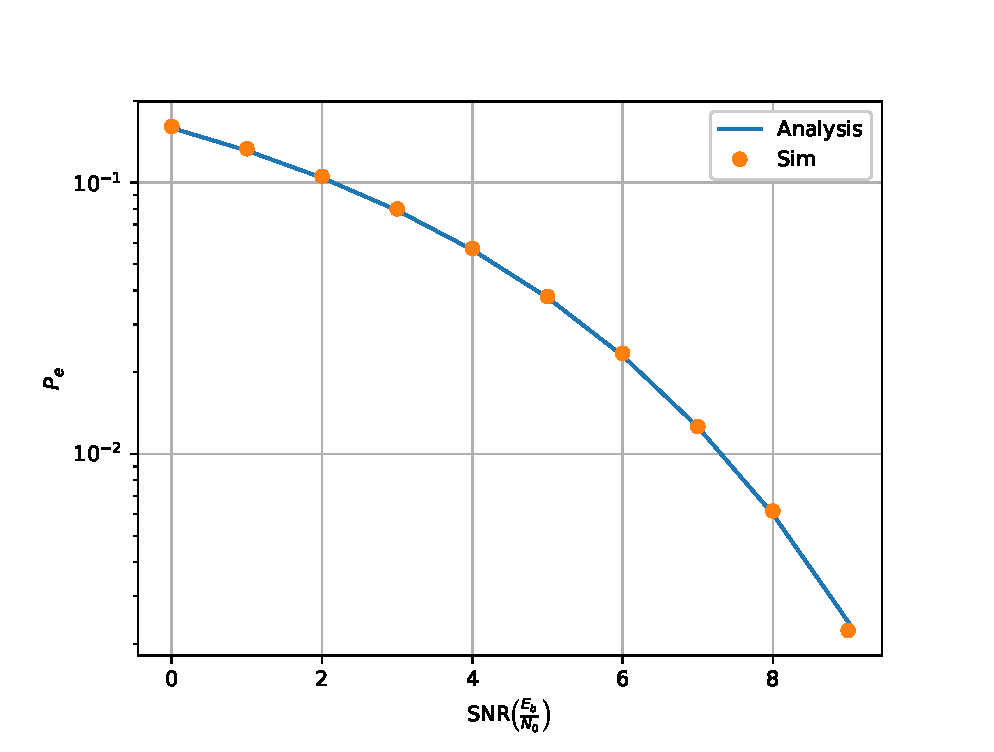
\includegraphics[width=\columnwidth]{./figs/bpsk_ber.eps}
\caption{}
\label{fig:ee18btech11042_bpsk_ber}
\end{figure}


\end{enumerate}

\section{Coherent BFSK}
\begin{enumerate}[label=\thesection.\arabic*.,ref=\thesection.\theenumi]
\numberwithin{equation}{enumi}

\item
The signal constellation for binary frequency shift keying (BFSK) is given in Fig. \ref{fig:ee18btech11042_bfsk_const}.
Obtain the equations for the received symbols.
\begin{figure}[!ht]
\centering
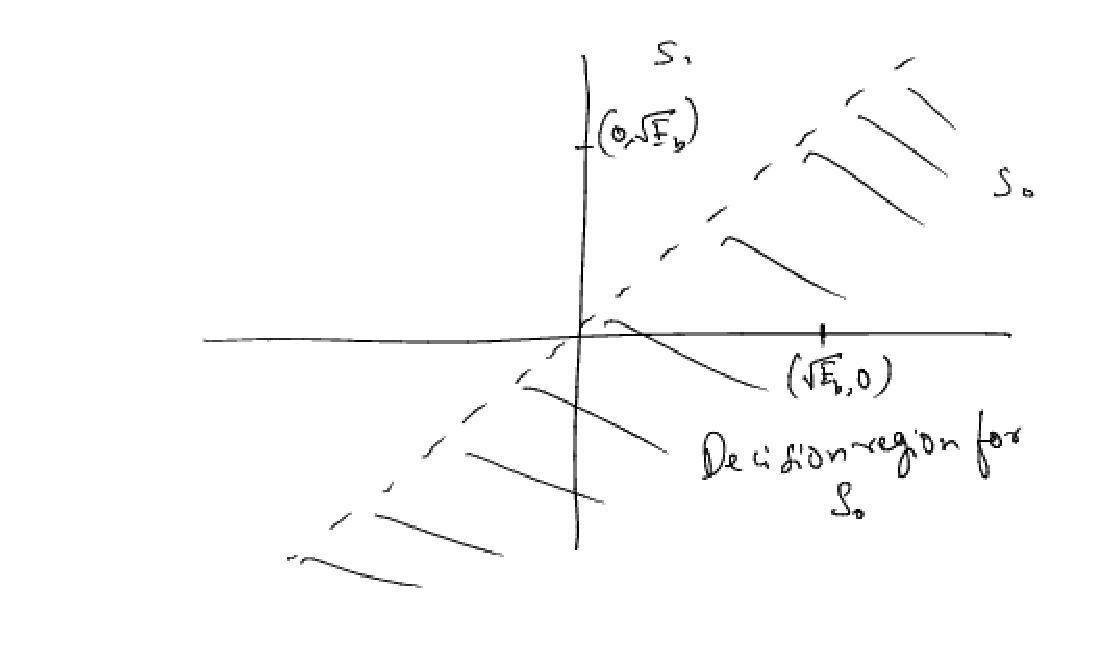
\includegraphics[width=\columnwidth]{./figs/bfsk_const.eps}
\caption{}
\label{fig:ee18btech11042_bfsk_const}
\end{figure}
\\
\solution
The received symbols are given by
\begin{align}
\mathbf{y}|s_0 = 
\begin{pmatrix*}
\sqrt{E_b} \\
0
\end{pmatrix*}
+
\begin{pmatrix*}
 n_{1}\\
n_{2}
\end{pmatrix*},
\end{align}
and 
\begin{align}
\mathbf{y}|s_1 = 
\begin{pmatrix*}
0\\
\sqrt{E_b} 
\end{pmatrix*}
+
\begin{pmatrix*}
n_{1}\\
 n_{2}
\end{pmatrix*},
\end{align}
where $n_1,n_2 \sim \gauss{0}{\frac{N_0}{2}}$. and
$
\mathbf{y} = 
\begin{pmatrix*}
y_{1}\\
 y_{2}
\end{pmatrix*}
$.

\item
Obtain a decision rule for BFSK from Fig. \ref{fig:ee18btech11042_bfsk_const}.
\solution The decision rule is
\begin{equation}
\label{eq:bfsk_dec}
y_1 \dec{s_0}{s_1} y_2
\end{equation}
\item The multivariate Gaussian distribution is defined as
%
\begin{multline}
\label{eq:multivariate}
p_{\mathbf{x}}(x_1,\dots,x_k)
\\
=\frac{1}{\sqrt{\brak{2\pi}^k\abs{\bm{\Sigma}}}}\exp\cbrak{-\frac{1}{2}\brak{\mathbf{x}-\bm{\mu}}^T\bm{\Sigma}^{-1}\brak{\mathbf{x}-\bm{\mu}}}
\end{multline}
%
where $\bm{\mu}$ is the mean vector, $\bm{\Sigma} = E\sbrak{\brak{\mathbf{x}-\bm{\mu}}\brak{\mathbf{x}-\bm{\mu}}^T}$ is the covariance matrix and $\abs{\bm{\Sigma}}$ is the determinant of $\bm{\Sigma}$.
Show that the PDF of the {\em bivariate} Gaussian is
{\small
\begin{multline}
\label{eq:bivariate}
p(x,y)= \frac{1}{2\pi \sigma_x\sigma_y\sqrt{1-\rho^2}}\exp\lsbrak{-\frac{1}{2\brak{1-\rho^2}}}
\\
\times \rsbrak{\cbrak{\frac{\brak{x-\mu_x}^2}{\sigma_x^2}+\frac{\brak{y-\mu_y}^2}{\sigma_y^2}-\frac{2\rho\brak{x-\mu_x}\brak{y-\mu_y}}{\sigma_x\sigma_y}}}
\end{multline}
}
%
where
%
\begin{align}
%\bm{\mu}=
\bm{\mu}=
\begin{pmatrix*}
\mu_x \\
\mu_y
\end{pmatrix*},
\bm{\Sigma} = 
\begin{pmatrix*}%[r]
\sigma_x^2 & \rho\sigma_x\sigma_y \\
\rho\sigma_x\sigma_y & \sigma_y^2
\end{pmatrix*}
\end{align}

%The multivariate Gaussian distribution is defined as
%%
%\begin{multline}
%p_{\mathbf{x}}(x_1,\dots,x_k)
%\\
%=\frac{1}{\sqrt{\brak{2\pi}^k\abs{\Sigma}}}\exp\cbrak{-\frac{1}{2}\brak{\mathbf{x}-\mathbf{\mu}}^T\Sigma^{-1}\brak{\mathbf{x}-\mathbf{\mu}}}
%\end{multline}
%%
%where $\mathbf{\mu}$ is the mean vector, $\Sigma = E\sbrak{\brak{\mathbf{x}-\mathbf{\mu}}\brak{\mathbf{x}-\mathbf{\mu}}^T}$ is the covariance matrix and $\abs{\Sigma}$ is the determinant of $\Sigma$.
%\begin{definition}
%The joint PDF of $X,Y$ is given by
%{\small
%\begin{multline}
%\label{eq:bivariate}
%p(x,y)= \frac{1}{2\pi \sigma_x\sigma_y\sqrt{1-\rho^2}}\exp\lsbrak{-\frac{1}{2\brak{1-\rho^2}}}
%\\
%\times \rsbrak{\cbrak{\frac{\brak{x-\mu_x}^2}{\sigma_x^2}+\frac{\brak{y-\mu_y}^2}{\sigma_y^2}-\frac{2\rho\brak{x-\mu_x}\brak{y-\mu_y}}{\sigma_x\sigma_y}}}
%\end{multline}
%}
%%
%where
%\begin{align}
%\mu_x &= E\sbrak{X},
%\\
%\sigma_x^2 &= \text{var}\brak{X},
%\\
%\rho &= \frac{E\sbrak{\brak{X - \mu_x}\brak{Y-\mu_y}}}{\sigma_x\sigma_y}.
%\end{align}
%%where
%%%
%%\begin{align}
%%\mathbf{\mu}=
%%\begin{pmatrix*}
%%\mu_x \\
%%\mu_y
%%\end{pmatrix*},
%%\Sigma = 
%%\begin{pmatrix*}%[r]
%%\sigma_x^2 & \rho\sigma_x\sigma_y \\
%%\rho\sigma_x\sigma_y & \sigma_y^2
%%\end{pmatrix*}
%%\end{align}
%%
%\end{definition}
%%

For equiprobably symbols, the MAP criterion is defined as
%
\begin{equation}
\label{eq:map_bfsk_dec}
%p\brak{\mathbf{y}|s_0} \dec{s_0}{s_1} p\brak{\mathbf{y}|s_1}
p\brak{s_0|\vec{y}} \dec{s_0}{s_1} p\brak{s_1|\vec{y}}
\end{equation}
\item
Use \eqref{eq:bivariate} in \eqref{eq:map_bfsk_dec}  to obtain \eqref{eq:bfsk_dec}.
\\
\solution According to the MAP criterion, assuming equiprobably symbols,
\begin{align}
%\pr{ \mathbf{y}|s_0 }
%p\brak{\mathbf{y}|s_0} \dec{s_0}{s_1} p\brak{\mathbf{y}|s_1}
p\brak{s_0|\vec{y}} \dec{s_0}{s_1} p\brak{s_1|\vec{y}}
\end{align}

\item
Derive and plot the probability of error.  Verify through simulation.
\\
\solution Given that $s_0$ was transmitted, the received symbols are
\begin{align}
\mathbf{y}|s_0 = 
\begin{pmatrix*}
\sqrt{E_b} \\
0
\end{pmatrix*}
+
\begin{pmatrix*}
 n_{1}\\
n_{2}
\end{pmatrix*},
\end{align}
From \eqref{eq:bfsk_dec}, 
the probability of error is given by
\begin{align}
P_e &= \pr{y_1 < y_2|s_0} = \pr{\sqrt{E_b} + n_1 < n_2}
\\
&= \pr{ n_2-n_1 > \sqrt{E_b} } 
\label{eq:bfsk_proof_n0}
\end{align}
Note that $n_2-n_1 \sim \gauss{0}{N_0}$. Thus, 
\begin{align}
P_e &= \pr{ \sqrt{N_0}w > \sqrt{E_b} }  
\\
&=  \pr{ w > \sqrt{\frac{E_b}{N_0}} }
%= \pr{ X > \sqrt{E_b} }
\\
\implies 
P_e & = \qfunc{\sqrt{\frac{E_b}{N_0}}}
\end{align}
where 
%$X \sim \gauss{0}{N_0}$
%\\
$w \sim \gauss{0}{1}$.  
%Then $X = \sqrt{N_0}w$. Substituting this in \eqref{eq:fsk_proof_n0},
%where $\qfunc{x} \define \pr{w > x}, x \ge 0$.
%
The following code plots the BER curves in Fig. \ref{fig:ee18btech11042_bfsk_ber}
\begin{lstlisting}
codes/fsk_ber.py
\end{lstlisting}
%
\begin{figure}[!ht]
\centering
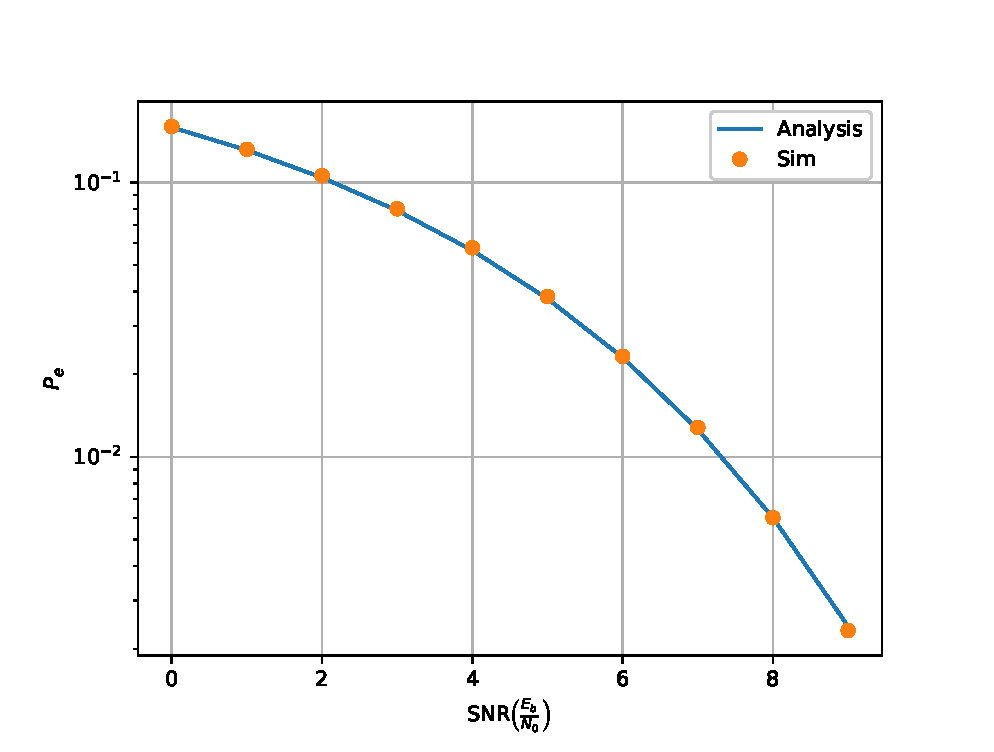
\includegraphics[width=\columnwidth]{./figs/bfsk_ber.eps}
\caption{}
\label{fig:ee18btech11042_bfsk_ber}
\end{figure}

\end{enumerate}
\section{QPSK}
\begin{enumerate}[label=\arabic*.,ref=\thesection.\theenumi]
\numberwithin{equation}{enumi}
%
\item See Fig.\ref{fig:ee18btech11041_fig1} for the constellation diagram.  The transmitted symbol set is given by 
\begin{align}
\vec{s}_m = \myvec{\cos \frac{2m\pi}{4}\\ \sin \frac{2m\pi}{4}}, \quad m \in \cbrak{0, 1, \dots, 3}.
%\vec{y = s + n}
\end{align}
%
The numerical values and encoding scheme for $\vec{s}_m$ are listed in Table \ref{table:ee18btech11041_table1}

\begin{figure}[!ht]
                \resizebox{\columnwidth}{!}{
\begin{tikzpicture}

\draw[<->,thick] (-4,0)--(4,0) node[right]{$\phi_1$};
\draw[<->,thick] (0,-4)--(0,4) node[above]{$\phi_2$};

\filldraw[black] (2.5,0) circle (2pt) node[below] {$s_0$} ;
\filldraw[black] (0,2.5) circle (2pt) node[left] {$s_1$} ;
\filldraw[black] (-2.5,0) circle (2pt) node[below] {$s_2$} ;
\filldraw[black] (0,-2.5) circle (2pt) node[left] {$s_3$} ;

\end{tikzpicture}
}

\caption{constellation diagram}
\label{fig:ee18btech11041_fig1}
\end{figure}
\begin{table}[!ht]
\centering
%%%%%%%%%%%%%%%%%%%%%%%%%%%%%%%%%%%%%%%%%%%%%%%%%%%%%%%%%%%%%%%%%%%%%%
%%                                                                  %%
%%  This is the header of a LaTeX2e file exported from Gnumeric.    %%
%%                                                                  %%
%%  This file can be compiled as it stands or included in another   %%
%%  LaTeX document. The table is based on the longtable package so  %%
%%  the longtable options (headers, footers...) can be set in the   %%
%%  preamble section below (see PRAMBLE).                           %%
%%                                                                  %%
%%  To include the file in another, the following two lines must be %%
%%  in the including file:                                          %%
%%        \def\inputGnumericTable{}                                 %%
%%  at the beginning of the file and:                               %%
%%        \input{name-of-this-file.tex}                             %%
%%  where the table is to be placed. Note also that the including   %%
%%  file must use the following packages for the table to be        %%
%%  rendered correctly:                                             %%
%%    \usepackage[latin1]{inputenc}                                 %%
%%    \usepackage{color}                                            %%
%%    \usepackage{array}                                            %%
%%    \usepackage{longtable}                                        %%
%%    \usepackage{calc}                                             %%
%%    \usepackage{multirow}                                         %%
%%    \usepackage{hhline}                                           %%
%%    \usepackage{ifthen}                                           %%
%%  optionally (for landscape tables embedded in another document): %%
%%    \usepackage{lscape}                                           %%
%%                                                                  %%
%%%%%%%%%%%%%%%%%%%%%%%%%%%%%%%%%%%%%%%%%%%%%%%%%%%%%%%%%%%%%%%%%%%%%%



%%  This section checks if we are begin input into another file or  %%
%%  the file will be compiled alone. First use a macro taken from   %%
%%  the TeXbook ex 7.7 (suggestion of Han-Wen Nienhuys).            %%
\def\ifundefined#1{\expandafter\ifx\csname#1\endcsname\relax}


%%  Check for the \def token for inputed files. If it is not        %%
%%  defined, the file will be processed as a standalone and the     %%
%%  preamble will be used.                                          %%
\ifundefined{inputGnumericTable}

%%  We must be able to close or not the document at the end.        %%
	\def\gnumericTableEnd{\end{document}}


%%%%%%%%%%%%%%%%%%%%%%%%%%%%%%%%%%%%%%%%%%%%%%%%%%%%%%%%%%%%%%%%%%%%%%
%%                                                                  %%
%%  This is the PREAMBLE. Change these values to get the right      %%
%%  paper size and other niceties.                                  %%
%%                                                                  %%
%%%%%%%%%%%%%%%%%%%%%%%%%%%%%%%%%%%%%%%%%%%%%%%%%%%%%%%%%%%%%%%%%%%%%%

	\documentclass[12pt%
			  %,landscape%
                    ]{report}
       \usepackage[latin1]{inputenc}
       \usepackage{fullpage}
       \usepackage{color}
       \usepackage{array}
       \usepackage{longtable}
       \usepackage{calc}
       \usepackage{multirow}
       \usepackage{hhline}
       \usepackage{ifthen}

	\begin{document}


%%  End of the preamble for the standalone. The next section is for %%
%%  documents which are included into other LaTeX2e files.          %%
\else

%%  We are not a stand alone document. For a regular table, we will %%
%%  have no preamble and only define the closing to mean nothing.   %%
    \def\gnumericTableEnd{}

%%  If we want landscape mode in an embedded document, comment out  %%
%%  the line above and uncomment the two below. The table will      %%
%%  begin on a new page and run in landscape mode.                  %%
%       \def\gnumericTableEnd{\end{landscape}}
%       \begin{landscape}


%%  End of the else clause for this file being \input.              %%
\fi

%%%%%%%%%%%%%%%%%%%%%%%%%%%%%%%%%%%%%%%%%%%%%%%%%%%%%%%%%%%%%%%%%%%%%%
%%                                                                  %%
%%  The rest is the gnumeric table, except for the closing          %%
%%  statement. Changes below will alter the table's appearance.     %%
%%                                                                  %%
%%%%%%%%%%%%%%%%%%%%%%%%%%%%%%%%%%%%%%%%%%%%%%%%%%%%%%%%%%%%%%%%%%%%%%

\providecommand{\gnumericmathit}[1]{#1} 
%%  Uncomment the next line if you would like your numbers to be in %%
%%  italics if they are italizised in the gnumeric table.           %%
%\renewcommand{\gnumericmathit}[1]{\mathit{#1}}
\providecommand{\gnumericPB}[1]%
{\let\gnumericTemp=\\#1\let\\=\gnumericTemp\hspace{0pt}}
 \ifundefined{gnumericTableWidthDefined}
        \newlength{\gnumericTableWidth}
        \newlength{\gnumericTableWidthComplete}
        \newlength{\gnumericMultiRowLength}
        \global\def\gnumericTableWidthDefined{}
 \fi
%% The following setting protects this code from babel shorthands.  %%
 \ifthenelse{\isundefined{\languageshorthands}}{}{\languageshorthands{english}}
%%  The default table format retains the relative column widths of  %%
%%  gnumeric. They can easily be changed to c, r or l. In that case %%
%%  you may want to comment out the next line and uncomment the one %%
%%  thereafter                                                      %%
\providecommand\gnumbox{\makebox[0pt]}
%%\providecommand\gnumbox[1][]{\makebox}

%% to adjust positions in multirow situations                       %%
\setlength{\bigstrutjot}{\jot}
\setlength{\extrarowheight}{\doublerulesep}

%%  The \setlongtables command keeps column widths the same across  %%
%%  pages. Simply comment out next line for varying column widths.  %%
\setlongtables

\setlength\gnumericTableWidth{%
	50pt+%
	70pt+%
	70pt+%
0pt}
\def\gumericNumCols{3}
\setlength\gnumericTableWidthComplete{\gnumericTableWidth+%
         \tabcolsep*\gumericNumCols*3+\arrayrulewidth*\gumericNumCols}
\ifthenelse{\lengthtest{\gnumericTableWidthComplete > \linewidth}}%
         {\def\gnumericScale{\ratio{\linewidth-%
                        \tabcolsep*\gumericNumCols*3-%
                        \arrayrulewidth*\gumericNumCols}%
{\gnumericTableWidth}}}%
{\def\gnumericScale{1}}

%%%%%%%%%%%%%%%%%%%%%%%%%%%%%%%%%%%%%%%%%%%%%%%%%%%%%%%%%%%%%%%%%%%%%%
%%                                                                  %%
%% The following are the widths of the various columns. We are      %%
%% defining them here because then they are easier to change.       %%
%% Depending on the cell formats we may use them more than once.    %%
%%                                                                  %%
%%%%%%%%%%%%%%%%%%%%%%%%%%%%%%%%%%%%%%%%%%%%%%%%%%%%%%%%%%%%%%%%%%%%%%

\ifthenelse{\isundefined{\gnumericColA}}{\newlength{\gnumericColA}}{}\settowidth{\gnumericColA}{\begin{tabular}{@{}p{50pt*\gnumericScale}@{}}x\end{tabular}}
\ifthenelse{\isundefined{\gnumericColB}}{\newlength{\gnumericColB}}{}\settowidth{\gnumericColB}{\begin{tabular}{@{}p{70pt*\gnumericScale}@{}}x\end{tabular}}
\ifthenelse{\isundefined{\gnumericColC}}{\newlength{\gnumericColC}}{}\settowidth{\gnumericColC}{\begin{tabular}{@{}p{70pt*\gnumericScale}@{}}x\end{tabular}}

\begin{tabular}[c]{%
	b{\gnumericColA}%
	b{\gnumericColB}%
	b{\gnumericColC}%
	}

%%%%%%%%%%%%%%%%%%%%%%%%%%%%%%%%%%%%%%%%%%%%%%%%%%%%%%%%%%%%%%%%%%%%%%
%%  The longtable options. (Caption, headers... see Goosens, p.124) %%
%	\caption{The Table Caption.}             \\	%
% \hline	% Across the top of the table.
%%  The rest of these options are table rows which are placed on    %%
%%  the first, last or every page. Use \multicolumn if you want.    %%

%%  Header for the first page.                                      %%
%	\multicolumn{2}{c}{The First Header} \\ \hline 
%	\multicolumn{1}{c}{colTag}	%Column 1
%	&\multicolumn{1}{c}{colTag}	\\ \hline %Last column
%	\endfirsthead

%%  The running header definition.                                  %%
%	\hline
%	\multicolumn{2}{l}{\ldots\small\slshape continued} \\ \hline
%	\multicolumn{1}{c}{colTag}	%Column 1
%	&\multicolumn{1}{c}{colTag}	\\ \hline %Last column
%	\endhead

%%  The running footer definition.                                  %%
%	\hline
%	\multicolumn{2}{r}{\small\slshape continued\ldots} \\
%	\endfoot

%%  The ending footer definition.                                   %%
%	\multicolumn{2}{c}{That's all folks} \\ \hline 
%	\endlastfoot
%%%%%%%%%%%%%%%%%%%%%%%%%%%%%%%%%%%%%%%%%%%%%%%%%%%%%%%%%%%%%%%%%%%%%%

\hhline{|-|-|-}
	 \multicolumn{1}{|p{\gnumericColA}|}%
	{\gnumericPB{\centering}\gnumbox{\textbf{Symbol}}}
	&\multicolumn{1}{p{\gnumericColB}|}%
	{\gnumericPB{\centering}\gnumbox{\textbf{Grey Code}}}
	&\multicolumn{1}{p{\gnumericColC}|}%
	{\gnumericPB{\centering}\gnumbox{\textbf{Co-ordinates}}}
\\


\hhline{|---|}
	 \multicolumn{1}{|p{\gnumericColA}|}%
	{\gnumericPB{\raggedright}\gnumbox[l]{$s_0$}}
	&\multicolumn{1}{p{\gnumericColB}|}%
	{\gnumericPB{\raggedright}\gnumbox[l]{$00$}}
    &\multicolumn{1}{p{\gnumericColC}|}%
	{\gnumericPB{\centering}\gnumbox{\myvec{1\\0 }}}
\\

\hhline{|---|}
	 \multicolumn{1}{|p{\gnumericColA}|}%
	{\gnumericPB{\raggedright}\gnumbox[l]{$s_1$}}
	&\multicolumn{1}{p{\gnumericColB}|}%
	{\gnumericPB{\raggedright}\gnumbox[l]{$01$}}
    &\multicolumn{1}{p{\gnumericColC}|}%
	{\gnumericPB{\centering}\gnumbox{\myvec{0\\1 }}}
\\

\hhline{|---|}
	 \multicolumn{1}{|p{\gnumericColA}|}%
	{\gnumericPB{\raggedright}\gnumbox[l]{$s_2$}}
	&\multicolumn{1}{p{\gnumericColB}|}%
	{\gnumericPB{\raggedright}\gnumbox[l]{$11$}}
    &\multicolumn{1}{p{\gnumericColC}|}%
	{\gnumericPB{\centering}\gnumbox{\myvec{-1\\ 0 }}}
\\

\hhline{|---|}
	 \multicolumn{1}{|p{\gnumericColA}|}%
	{\gnumericPB{\raggedright}\gnumbox[l]{$s_3$}}
	&\multicolumn{1}{p{\gnumericColB}|}%
	{\gnumericPB{\raggedright}\gnumbox[l]{$10$}}
    &\multicolumn{1}{p{\gnumericColC}|}%
	{\gnumericPB{\centering}\gnumbox{\myvec{0\\-1 }}}
\\
\hhline{|-|-|-|}
\end{tabular}

\ifthenelse{\isundefined{\languageshorthands}}{}{\languageshorthands{\languagename}}
\gnumericTableEnd
\caption{}
\label{table:ee18btech11041_table1}
\end{table}
\item Let
\begin{equation}
\label{eq:qpsk_rx}
\mathbf{y} = \sqrt{E}_s\mathbf{s}+ \mathbf{n}
\end{equation}
where $\mathbf{s} \in \cbrak{\mathbf{s}_0,\mathbf{s}_1,\mathbf{s}_2, \mathbf{s}_3}$ 
%
\item Obtain the decision rule for QPSK by inspection.
\\
\solution The decision rule is given by Fig.\ref{fig:ee18btech11041_fig2} 

\begin{figure}[!ht]
                \resizebox{\columnwidth}{!}{
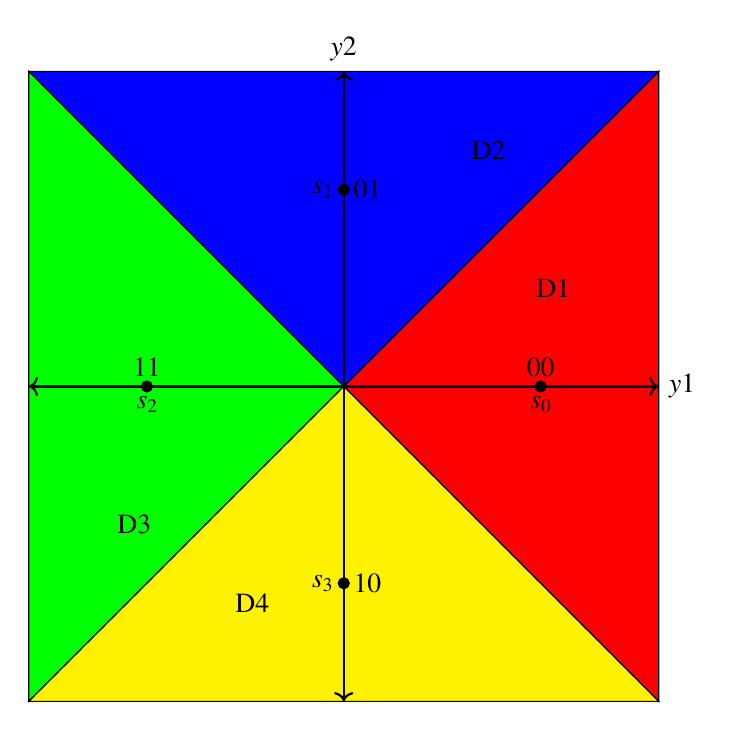
\begin{tikzpicture}


\draw[fill=red]  (0,0) -- (4,4) -- (4,-4)  -- cycle;

\draw[fill=blue]  (0,0) -- (4,4) -- (-4,4)  -- cycle;
\draw[fill=green]  (0,0) -- (-4,4) -- (-4,-4)  -- cycle;
\draw[fill=yellow]  (0,0) -- (-4,-4) -- (4,-4)  -- cycle;



\draw[<->,thick] (-4,0)--(4,0) node[right]{$y1$};
\draw[<->,thick] (0,-4)--(0,4) node[above]{$y2$};
\draw [dashed]   (-4,-4)--(4,4);
\draw [dashed]   (-4,4)--(4,-4);

\filldraw[black] (2.5,0) circle (2pt) node[below] {$s_0$} node[above] {00};
\filldraw[black] (0,2.5) circle (2pt) node[left] {$s_1$} node[right] {01};
\filldraw[black] (-2.5,0) circle (2pt) node[below] {$s_2$} node[above] {11};
\filldraw[black] (0,-2.5) circle (2pt) node[left] {$s_3$} node [right] {10} ;


\foreach \coordinate/\label/\pos in {{(3,1)/D1/above left},{(1.5,3)/D2/right},{(-3,-2)/D3/above right},{(-1.5,-3)/D4/above right}} \node[\pos] at \coordinate {\label};

\end{tikzpicture}
}
\caption{decision regions}
\label{fig:ee18btech11041_fig2}	
\end{figure}
\item Using \eqref{eq:bivariate}, show that the MAP decision for detecting $\vec{s}_0$ results in
\begin{equation}
\label{eq:qpsk_dec}
\abs{y_2} < y_1
\end{equation}
\solution The MAP criterion reduces to 
%
\begin{align}
    \hat{s} = \min_{\vec{s} \in \vec{s}_i} \norm{\vec{y} - \vec{s}}, i \in \cbrak{0,\dots,3}
    \label{eq:ee18btech11041_eq1}
\end{align}
%
From eq.\ref{eq:ee18btech11041_eq1},$\vec{s}_{0}$ is chosen if

\begin{align}
    \norm{\vec{y}-\vec{s}_0}^2 &< \norm{\vec{y}-\vec{s}_i}^2
\\
\implies    (\vec{s}_0-\vec{s}_i)^T\vec{y}&>0 \quad i \in \cbrak{1,2,3}
\end{align}
%\begin{align}
%    \norm{\vec{y}-\vec{s}_0}^2 < \norm{\vec{y}-\vec{s}_2}^2
%\end{align}
%\begin{align}
%    \norm{\vec{y}-\vec{s}_0}^2 < \norm{\vec{y}-\vec{s}_3}^2
%\end{align}
%


%\begin{align}
%    (\vec{s}_0-\vec{s}_1)^T\vec{y}>0
%\end{align}
%\begin{align}
%    (\vec{s}_0-\vec{s}_2)^T\vec{y}>0
%\end{align}
%\begin{align}
%    (\vec{s}_0-\vec{s}_3)^T\vec{y}>0
%\end{align}
%
%Substituting the values of $s_{0}$,$s_{1}$,....$s_{7}$ in the above
or,
\begin{align}
\myvec{1 & -1 \\ 1& 0 \\ 1 & 1}\vec{y}\succeq 0
\end{align}
The above condition can be simplified to obtain the region
\begin{align}
D_1: \abs{y_2}< y_1
\label{eq:qpsk_s0}
\end{align}
Table \ref{table:ee18btech11041_table2} summarizes the decisions for all symbols.
%
%
\begin{table}[!ht]
\centering
%%%%%%%%%%%%%%%%%%%%%%%%%%%%%%%%%%%%%%%%%%%%%%%%%%%%%%%%%%%%%%%%%%%%%%
%%                                                                  %%
%%  This is the header of a LaTeX2e file exported from Gnumeric.    %%
%%                                                                  %%
%%  This file can be compiled as it stands or included in another   %%
%%  LaTeX document. The table is based on the longtable package so  %%
%%  the longtable options (headers, footers...) can be set in the   %%
%%  preamble section below (see PRAMBLE).                           %%
%%                                                                  %%
%%  To include the file in another, the following two lines must be %%
%%  in the including file:                                          %%
%%        \def\inputGnumericTable{}                                 %%
%%  at the beginning of the file and:                               %%
%%        \input{name-of-this-file.tex}                             %%
%%  where the table is to be placed. Note also that the including   %%
%%  file must use the following packages for the table to be        %%
%%  rendered correctly:                                             %%
%%    \usepackage[latin1]{inputenc}                                 %%
%%    \usepackage{color}                                            %%
%%    \usepackage{array}                                            %%
%%    \usepackage{longtable}                                        %%
%%    \usepackage{calc}                                             %%
%%    \usepackage{multirow}                                         %%
%%    \usepackage{hhline}                                           %%
%%    \usepackage{ifthen}                                           %%
%%  optionally (for landscape tables embedded in another document): %%
%%    \usepackage{lscape}                                           %%
%%                                                                  %%
%%%%%%%%%%%%%%%%%%%%%%%%%%%%%%%%%%%%%%%%%%%%%%%%%%%%%%%%%%%%%%%%%%%%%%



%%  This section checks if we are begin input into another file or  %%
%%  the file will be compiled alone. First use a macro taken from   %%
%%  the TeXbook ex 7.7 (suggestion of Han-Wen Nienhuys).            %%
\def\ifundefined#1{\expandafter\ifx\csname#1\endcsname\relax}


%%  Check for the \def token for inputed files. If it is not        %%
%%  defined, the file will be processed as a standalone and the     %%
%%  preamble will be used.                                          %%
\ifundefined{inputGnumericTable}

%%  We must be able to close or not the document at the end.        %%
	\def\gnumericTableEnd{\end{document}}


%%%%%%%%%%%%%%%%%%%%%%%%%%%%%%%%%%%%%%%%%%%%%%%%%%%%%%%%%%%%%%%%%%%%%%
%%                                                                  %%
%%  This is the PREAMBLE. Change these values to get the right      %%
%%  paper size and other niceties.                                  %%
%%                                                                  %%
%%%%%%%%%%%%%%%%%%%%%%%%%%%%%%%%%%%%%%%%%%%%%%%%%%%%%%%%%%%%%%%%%%%%%%

	\documentclass[12pt%
			  %,landscape%
                    ]{report}
       \usepackage[latin1]{inputenc}
       \usepackage{fullpage}
       \usepackage{color}
       \usepackage{array}
       \usepackage{longtable}
       \usepackage{calc}
       \usepackage{multirow}
       \usepackage{hhline}
       \usepackage{ifthen}

	\begin{document}


%%  End of the preamble for the standalone. The next section is for %%
%%  documents which are included into other LaTeX2e files.          %%
\else

%%  We are not a stand alone document. For a regular table, we will %%
%%  have no preamble and only define the closing to mean nothing.   %%
    \def\gnumericTableEnd{}

%%  If we want landscape mode in an embedded document, comment out  %%
%%  the line above and uncomment the two below. The table will      %%
%%  begin on a new page and run in landscape mode.                  %%
%       \def\gnumericTableEnd{\end{landscape}}
%       \begin{landscape}


%%  End of the else clause for this file being \input.              %%
\fi

%%%%%%%%%%%%%%%%%%%%%%%%%%%%%%%%%%%%%%%%%%%%%%%%%%%%%%%%%%%%%%%%%%%%%%
%%                                                                  %%
%%  The rest is the gnumeric table, except for the closing          %%
%%  statement. Changes below will alter the table's appearance.     %%
%%                                                                  %%
%%%%%%%%%%%%%%%%%%%%%%%%%%%%%%%%%%%%%%%%%%%%%%%%%%%%%%%%%%%%%%%%%%%%%%

\providecommand{\gnumericmathit}[1]{#1} 
%%  Uncomment the next line if you would like your numbers to be in %%
%%  italics if they are italizised in the gnumeric table.           %%
%\renewcommand{\gnumericmathit}[1]{\mathit{#1}}
\providecommand{\gnumericPB}[1]%
{\let\gnumericTemp=\\#1\let\\=\gnumericTemp\hspace{0pt}}
 \ifundefined{gnumericTableWidthDefined}
        \newlength{\gnumericTableWidth}
        \newlength{\gnumericTableWidthComplete}
        \newlength{\gnumericMultiRowLength}
        \global\def\gnumericTableWidthDefined{}
 \fi
%% The following setting protects this code from babel shorthands.  %%
 \ifthenelse{\isundefined{\languageshorthands}}{}{\languageshorthands{english}}
%%  The default table format retains the relative column widths of  %%
%%  gnumeric. They can easily be changed to c, r or l. In that case %%
%%  you may want to comment out the next line and uncomment the one %%
%%  thereafter                                                      %%
\providecommand\gnumbox{\makebox[0pt]}
%%\providecommand\gnumbox[1][]{\makebox}

%% to adjust positions in multirow situations                       %%
\setlength{\bigstrutjot}{\jot}
\setlength{\extrarowheight}{\doublerulesep}

%%  The \setlongtables command keeps column widths the same across  %%
%%  pages. Simply comment out next line for varying column widths.  %%
\setlongtables

\setlength\gnumericTableWidth{%
	40pt+%
	70pt+%
	85pt+%
0pt}
\def\gumericNumCols{3}
\setlength\gnumericTableWidthComplete{\gnumericTableWidth+%
         \tabcolsep*\gumericNumCols*3+\arrayrulewidth*\gumericNumCols}
\ifthenelse{\lengthtest{\gnumericTableWidthComplete > \linewidth}}%
         {\def\gnumericScale{\ratio{\linewidth-%
                        \tabcolsep*\gumericNumCols*3-%
                        \arrayrulewidth*\gumericNumCols}%
{\gnumericTableWidth}}}%
{\def\gnumericScale{1}}

%%%%%%%%%%%%%%%%%%%%%%%%%%%%%%%%%%%%%%%%%%%%%%%%%%%%%%%%%%%%%%%%%%%%%%
%%                                                                  %%
%% The following are the widths of the various columns. We are      %%
%% defining them here because then they are easier to change.       %%
%% Depending on the cell formats we may use them more than once.    %%
%%                                                                  %%
%%%%%%%%%%%%%%%%%%%%%%%%%%%%%%%%%%%%%%%%%%%%%%%%%%%%%%%%%%%%%%%%%%%%%%

\ifthenelse{\isundefined{\gnumericColA}}{\newlength{\gnumericColA}}{}\settowidth{\gnumericColA}{\begin{tabular}{@{}p{40pt*\gnumericScale}@{}}x\end{tabular}}
\ifthenelse{\isundefined{\gnumericColB}}{\newlength{\gnumericColB}}{}\settowidth{\gnumericColB}{\begin{tabular}{@{}p{70pt*\gnumericScale}@{}}x\end{tabular}}
\ifthenelse{\isundefined{\gnumericColC}}{\newlength{\gnumericColC}}{}\settowidth{\gnumericColC}{\begin{tabular}{@{}p{85pt*\gnumericScale}@{}}x\end{tabular}}

\begin{tabular}[c]{%
	b{\gnumericColA}%
	b{\gnumericColB}%
	b{\gnumericColC}%
	}

%%%%%%%%%%%%%%%%%%%%%%%%%%%%%%%%%%%%%%%%%%%%%%%%%%%%%%%%%%%%%%%%%%%%%%
%%  The longtable options. (Caption, headers... see Goosens, p.124) %%
%	\caption{The Table Caption.}             \\	%
% \hline	% Across the top of the table.
%%  The rest of these options are table rows which are placed on    %%
%%  the first, last or every page. Use \multicolumn if you want.    %%

%%  Header for the first page.                                      %%
%	\multicolumn{2}{c}{The First Header} \\ \hline 
%	\multicolumn{1}{c}{colTag}	%Column 1
%	&\multicolumn{1}{c}{colTag}	\\ \hline %Last column
%	\endfirsthead

%%  The running header definition.                                  %%
%	\hline
%	\multicolumn{2}{l}{\ldots\small\slshape continued} \\ \hline
%	\multicolumn{1}{c}{colTag}	%Column 1
%	&\multicolumn{1}{c}{colTag}	\\ \hline %Last column
%	\endhead

%%  The running footer definition.                                  %%
%	\hline
%	\multicolumn{2}{r}{\small\slshape continued\ldots} \\
%	\endfoot

%%  The ending footer definition.                                   %%
%	\multicolumn{2}{c}{That's all folks} \\ \hline 
%	\endlastfoot
%%%%%%%%%%%%%%%%%%%%%%%%%%%%%%%%%%%%%%%%%%%%%%%%%%%%%%%%%%%%%%%%%%%%%%

\hhline{|-|-|-}
	 \multicolumn{1}{|p{\gnumericColA}|}%
	{\gnumericPB{\centering}\gnumbox{\textbf{Symbol}}}
	&\multicolumn{1}{p{\gnumericColB}|}%
	{\gnumericPB{\centering}\gnumbox{\textbf{Decision region}}}
	&\multicolumn{1}{p{\gnumericColC}|}%
	{\gnumericPB{\centering}\gnumbox{\textbf{Decision Rule}}}
\\


\hhline{|---|}
	 \multicolumn{1}{|p{\gnumericColA}|}%
	{\gnumericPB{\raggedright}\gnumbox[l]{$s_0$}}
	&\multicolumn{1}{p{\gnumericColB}|}%
	{\gnumericPB{\raggedright}\gnumbox[l]{$D1$}}
    &\multicolumn{1}{p{\gnumericColC}|}%
	{\gnumericPB{\centering}\gnumbox{ $y1>y2 , y1>-y2$}}
\\

\hhline{|---|}
	 \multicolumn{1}{|p{\gnumericColA}|}%
	{\gnumericPB{\raggedright}\gnumbox[l]{$s_1$}}
	&\multicolumn{1}{p{\gnumericColB}|}%
	{\gnumericPB{\raggedright}\gnumbox[l]{$D2$}}
    &\multicolumn{1}{p{\gnumericColC}|}%
	{\gnumericPB{\centering}\gnumbox{$y1<y2,y1>-y2$}}
\\

\hhline{|---|}
	 \multicolumn{1}{|p{\gnumericColA}|}%
	{\gnumericPB{\raggedright}\gnumbox[l]{$s_2$}}
	&\multicolumn{1}{p{\gnumericColB}|}%
	{\gnumericPB{\raggedright}\gnumbox[l]{$D3$}}
    &\multicolumn{1}{p{\gnumericColC}|}%
	{\gnumericPB{\centering}\gnumbox{$y1<y2,y1<-y2$}}
\\

\hhline{|---|}
	 \multicolumn{1}{|p{\gnumericColA}|}%
	{\gnumericPB{\raggedright}\gnumbox[l]{$s_3$}}
	&\multicolumn{1}{p{\gnumericColB}|}%
	{\gnumericPB{\raggedright}\gnumbox[l]{$D3$}}
    &\multicolumn{1}{p{\gnumericColC}|}%
	{\gnumericPB{\centering}\gnumbox{$y1>y2,y1<-y2$}}
\\
\hhline{|-|-|-|}
\end{tabular}

\ifthenelse{\isundefined{\languageshorthands}}{}{\languageshorthands{\languagename}}
\gnumericTableEnd
\caption{}
\label{table:ee18btech11041_table2}
\end{table}


\item Express $\pr{\hat{\mathbf{s}} = \mathbf{s}_0|\mathbf{s} = \mathbf{s}_0}$ in terms of 
$y_1, y_2$.
\\
\solution From \eqref{eq:qpsk_dec} and \eqref{eq:qpsk_s0}
,
\begin{multline}
\label{eq:ser_dec}
\pr{\hat{\mathbf{s}} = \mathbf{s}_0|\mathbf{s} = \mathbf{s}_0} 
\\
= \pr{\abs{y_2} < y_1
|y_1 = \sqrt{E}_s, y_2 = 0}
\end{multline}
%$r_1, r_2$.
\item Let 
\label{prob:qpsk_xy}
\begin{align}
\label{eq:qpskx}
X=n_2-n_1, 
\\
Y = -n_2-n_1, 
\label{eq:qpsky}
\end{align}
where $\mathbf{n}=\myvec{n_1\\n_2}$.

Show that $X,Y \sim \mathcal{N}\brak{0,N_0}$.

\item The correlation coefficient of $X, Y$ is defined as
%
\begin{align}
\rho = \frac{E\sbrak{\brak{X-\mu_x}\brak{Y-\mu_y}}}{\sigma_x\sigma_y}
\end{align}
%
$X$ and $Y$ are said to be uncorrelated if $\rho = 0$
Show that  $X$ and $Y$ are uncorrelated. 
Verify this numerically.
\\
\solution From \eqref{eq:qpskx}
and \eqref{eq:qpsky}
%\eqref{eq:qpsk_mean},
\begin{align}
\mu_x &= E\sbrak{X} = 0
\\
\mu_y &= E\sbrak{Y} = 0
\\
\implies \rho &= E\sbrak{XY} = E\sbrak{\brak{n_2-n_1}\brak{-n_2-n_1}} 
\nonumber \\
&= 0
\label{eq:qpsk_uncorr}
\end{align}
%
upon substituting from \eqref{eq:qpskx} and \eqref{eq:qpsky}.
\item
Show that $X$ and $Y$ are independent, i.e. 
\begin{align}
\label{eq:qpsk_uncorr_indep}
p_{XY}(x,y) = p_{X}(x)p_{Y}(y).
\end{align}
\\
\solution Use \eqref{eq:qpsk_uncorr} in 
\eqref{eq:bivariate} to get \eqref{eq:qpsk_uncorr_indep}.  Uncorrelated Gaussians are independent.

\item

Show that 
\begin{equation}
\pr{\hat{\mathbf{s}} = \mathbf{s}_0|\mathbf{s} = \mathbf{s}_0} =\pr{ X < \sqrt{E_s}}\pr{  Y < \sqrt{E_s}}.
\end{equation}
\\
\solution From \eqref{eq:ser_dec}  and \eqref{eq:qpsk_rx}
%and \eqref{eq:qpsk_s0}
%
\begin{multline}
\pr{\hat{\mathbf{s}} = \mathbf{s}_0|\mathbf{s} = \mathbf{s}_0} 
\\
= \pr{\abs{n_2} < \sqrt{E}_s+n_1}
\end{multline}
%
which can be expressed as
%
\begin{align}
\pr{{n_2} < \sqrt{E}_s+n_1,-{n_2} > \sqrt{E}_s+n_1 }&
\\
= \pr{X < \sqrt{E}_s,Y < \sqrt{E}_s }&
\\
=\pr{X < \sqrt{E}_s}\pr{Y < \sqrt{E}_s }&
\end{align}
%
after some algebra, using the fact that $X,Y$ are independent.
\item

Show that 
\begin{equation}
\pr{\hat{\mathbf{s}} = \mathbf{s}_0|\mathbf{s} = \mathbf{s}_0} 
 = \brak{1-\qfunc{\sqrt{\frac{E_s}{N_0}}}}^2
\label{eq:qpsk_ser_final}
\end{equation}
\solution From \eqref{prob:qpsk_xy}, 
\begin{align}
\pr{X > \sqrt{E}_s} = \pr{Y > \sqrt{E}_s} = \qfunc{\sqrt{\frac{E_s}{N_0}}}
\end{align}
yielding \eqref{eq:qpsk_ser_final}.

\item

Verify the above through simulation.
\\
\solution 
This is shown in Fig. \ref{fig:ee18btech11042_qpsk} through the following code.
\begin{lstlisting}
codes/qpsk.py
\end{lstlisting}
%
\begin{figure}[!ht]
\centering
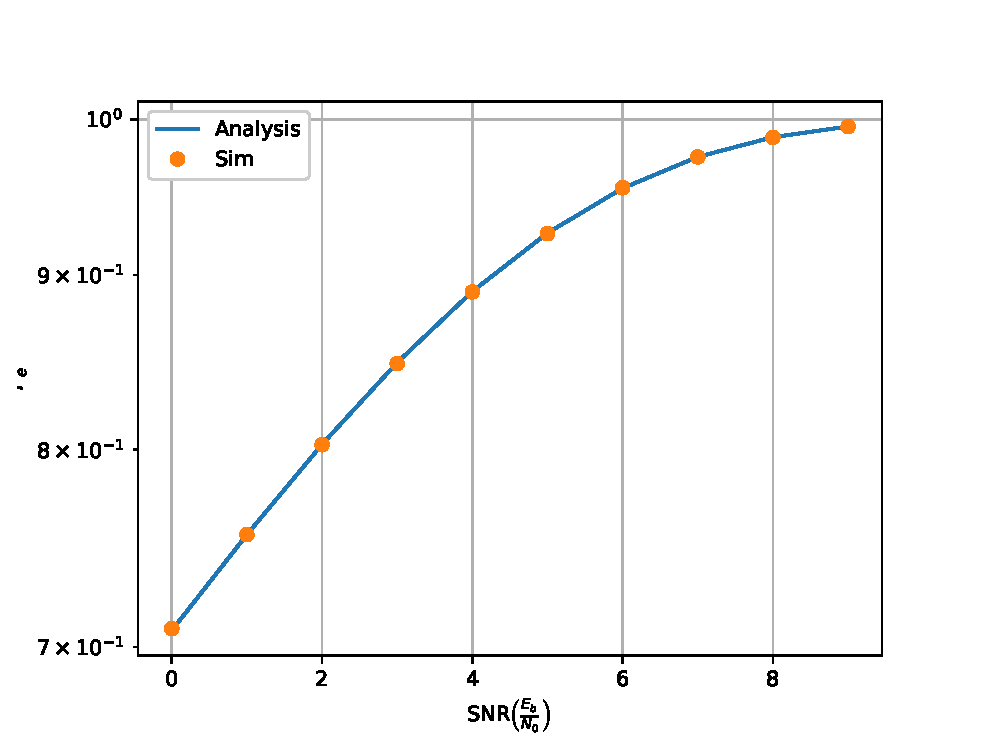
\includegraphics[width=\columnwidth]{./figs/qpsk.eps}
\caption{}
\label{fig:ee18btech11042_qpsk}
\end{figure}

\item
Modify the above script to obtain the probability of symbol error.

%\begin{enumerate}
%\item 
%\item 
%\item 
%\item 
%\item 
%\item 
%\\
%\solution Given we transmitted $s_0$, the probability of decoding it as $s_0$ is given by 
%\begin{equation}
%\pr{\hat{\mathbf{s}} = \mathbf{s}_0|\mathbf{s} = \mathbf{s}_0} = \pr{-n_2<\sqrt{E_s}+n_1,\sqrt{E_s}+n_1>n_2} 
%\end{equation}
%\begin{equation}
%\implies \pr{\hat{\mathbf{s}} = \mathbf{s}_0|\mathbf{s} = \mathbf{s}_0} = \pr{X<\sqrt{E_s},Y<\sqrt{E_s}}
%\end{equation}
%\\
%Where, $X=n_2-n_1, Y=-n_2-n_1$. Also $X,Y \sim \mathcal{N}\brak{0,2\sigma^2}$ and are independent. 
%\item Show that 
%\begin{equation}
%\pr{ X < \sqrt{E_s},  Y < \sqrt{E_s}} = \brak{1-\qfunc{\sqrt{\frac{E_s}{N_0}}}}^2
%\end{equation}
%\solution 
%\begin{equation}
%\pr{X < A, Y < A} = \pr{X < A}\pr{Y < A}
%\end{equation}
%\begin{equation}
%\implies \pr{X < A, Y < A} = \brak{1-\qfunc{\frac{A}{\sqrt{2}\sigma}}}^2
%\end{equation}
%\item 
%\\
%
%\item 
\end{enumerate}
%\item
\section{$M$-PSK}
\begin{enumerate}[label=\arabic*.,ref=\thesection.\theenumi]
\numberwithin{equation}{enumi}

\item Consider a system where 
$\mathbf{s}_i=
\begin{pmatrix}
\cos\brak{\frac{2\pi i}{M}}\\
\sin\brak{\frac{2\pi i}{M}}
\end{pmatrix}, i = 0, 1 , \dots M-1
$
.
Let
%
\begin{align}
\mathbf{y}|s_0 = 
\begin{pmatrix}
y_1\\
y_2
\end{pmatrix}
=
\begin{pmatrix}
\sqrt{E_s}+n_1\\
n_2
\end{pmatrix}
\end{align}
where $n_1,n_2 \sim \mathcal{N}\brak{0,\frac{N_0}{2}}$.

 Substituting 
\begin{align}
y_1=R\cos \theta \\
y_2=R\sin \theta
\end{align}
show that the joint pdf of $R,\theta$ is
%
\begin{equation}
p\brak{R,\theta}=\frac{R}{\pi N_0}\exp\brak{-\frac{R^2-2R\sqrt{E_s}\cos \theta + E_s}{N_0}}
\end{equation}
\item

Show that 
%
\begin{align}
\label{eq:mpsk_alpha1}
\lim_{\alpha \rightarrow \infty}\int_{0}^{\infty}\brak{V-\alpha }e^{-\brak{V-\alpha}^2 }\,dV
&= 0
\\
\label{eq:mpsk_alpha2}
\lim_{\alpha \rightarrow \infty}\int_{0}^{\infty} e^{-\brak{V-\alpha}^2 }\,dV
&=  \sqrt{\pi}
\end{align}
\item

Using the above, show that
%
\begin{multline}
\label{eq:mpsk_integ}
\int_{0}^{\infty}V\exp\cbrak{-\brak{V^2 - 2V \sqrt{\gamma}\cos \theta +\gamma}}\,dV
\\
= e^{-\gamma\sin^2 \theta} \sqrt{\gamma\pi}\cos \theta
%\label{eq:mpsk_gamma_large}
\end{multline}
%
for large values of $\gamma$.
\\
\solution The integrand in \eqref{eq:mpsk_integ} can be expressed as
\begin{multline}
Ve^{-\brak{V^2 - 2V \sqrt{\gamma}\cos \theta +\gamma}} 
\\
= \cbrak{\brak{V - \sqrt{\gamma}\cos \theta} + \brak{\sqrt{\gamma}\cos \theta}}
\\
\times e^{-\brak{V -  \sqrt{\gamma}\cos \theta }^2}e^{-  \sqrt{\gamma}\sin^2 \theta} 
\\
\implies \int_{0}^{\infty}Ve^{-\brak{V^2 - 2V \sqrt{\gamma}\cos \theta +\gamma}}\,dV
\\
 = e^{-  \sqrt{\gamma}\sin^2 \theta}
\\
\times  \lcbrak{\int_{0}^{\infty}\brak{V - \sqrt{\gamma}\cos \theta}e^{-\brak{V -  \sqrt{\gamma}\cos \theta }^2}\,d\theta}
\\
+ \rcbrak{\int_{0}^{\infty}\brak{\sqrt{\gamma}\cos \theta}e^{-\brak{V -  \sqrt{\gamma}\cos \theta }^2}\,d \theta}
\end{multline}
%
yielding \eqref{eq:mpsk_integ} from \eqref{eq:mpsk_alpha1}
and \eqref{eq:mpsk_alpha2}


\item

Find a compact expression for
%
\begin{align}
I = 1 - \sqrt{\frac{\gamma}{\pi}}\int_{-\frac{\pi}{M}}^{\frac{\pi}{M}}e^{- \gamma\sin^2\theta }\cos \theta\, d\theta
\end{align}
\solution The above integral can be expressed as
%
\begin{align}
I &= 1 - 2\sqrt{\frac{\gamma}{\pi}}\int_{0}^{\frac{\pi}{M}}e^{- \gamma\sin^2\theta }\cos \theta\, d\theta
\\
&= 1 - 2 \cbrak{\qfunc{0}-\qfunc{\sqrt{2\gamma}\sin \frac{\pi}{M}}}
\\
&= 2\qfunc{\sqrt{2\gamma}\sin \frac{\pi}{M}}
\end{align}
$\because \qfunc{0} = \frac{1}{2}$.
\item Find the decision region for the symbol $\vec{s}_0$.

\item

Show that
\begin{equation}
P_{e|\mathbf{s}_0}=2\qfunc{\sqrt{2\brak{\frac{{E_s}}{N_oN_0}}}\sin \frac{\pi}{M}}
\end{equation}
\item

Verify the SER through simulation.
\end{enumerate}
%
\end{document}


